Fig. \ref{fig:amino_acid_composition} compares the amino acid composition.
Some very similar preferences were observed in the Gammaproteobacteria when compared to \textit{Escherichia coli} as reported by \cite{loos2019}.
Cytoplasmic proteins are enriched in 
charged, and larger acyclic hydrophobic residues (Leu and Ile).
Periplasmic proteins on the other hand display a preference for polar and small hydrophobic residues (Ala, Val).
There are also some differences:
where \cite{loos2019} observed a preference for aromatic residues in the cytoplasmome,
this is not the case for this dataset.
However, it should be noted that this dataset only comprises periplasmic proteins,
whereas their set also contained those proteins that are fully excreted in the surrounding milieu.


~\begin{figure}[h!]
	\centering
	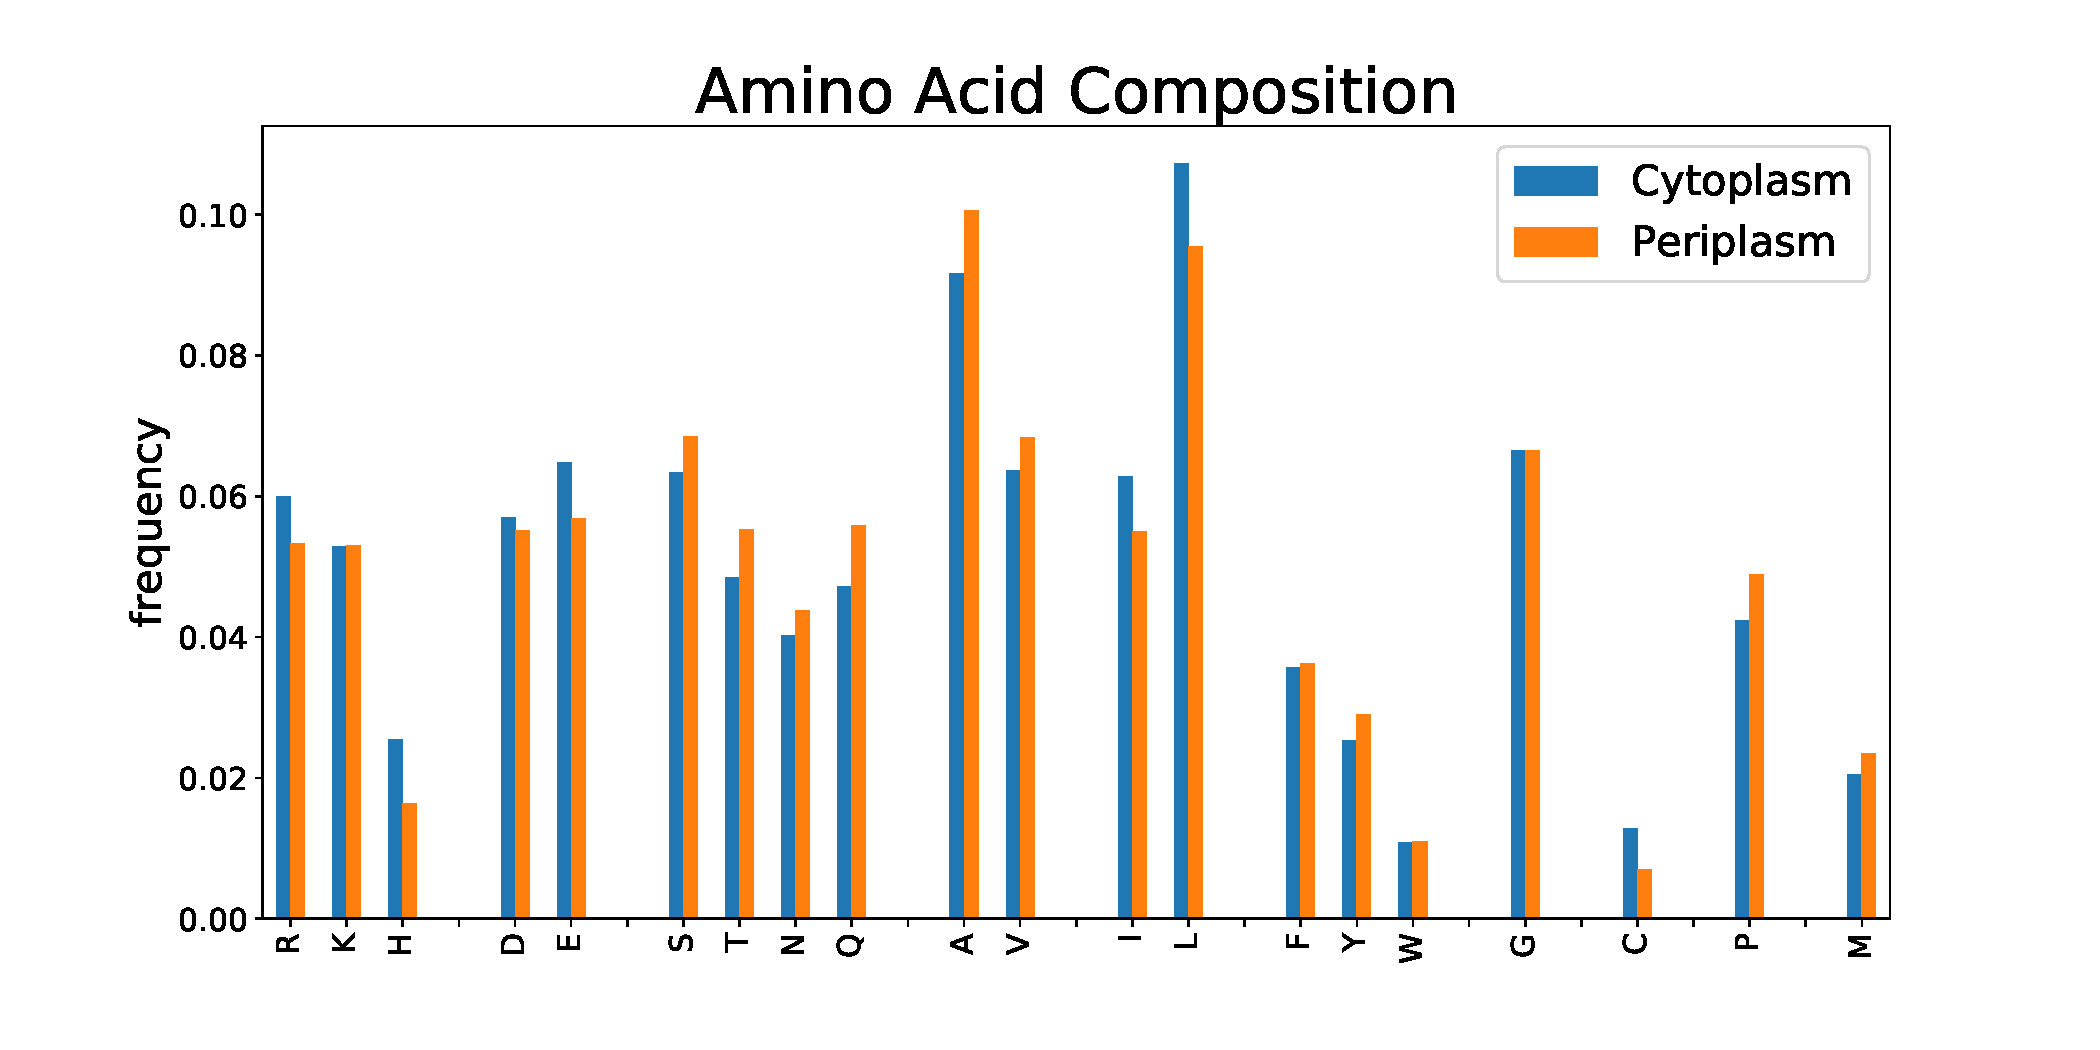
\includegraphics[width=\linewidth]{./results/general_comparison/global_comparison/amino_acid_composition/img/amino_acid_composition.pdf}
	\caption{\textbf{Amino acid composition in periplasmic and cytoplasmic proteins.}}
	\label{fig:amino_acid_composition}
~\end{figure}
